\section{Application Case---Fukushima Daiichi Reactor} \label{sec:cases}
\begin{figure}
    \centering
    \framebox[0.4\columnwidth][c]{
        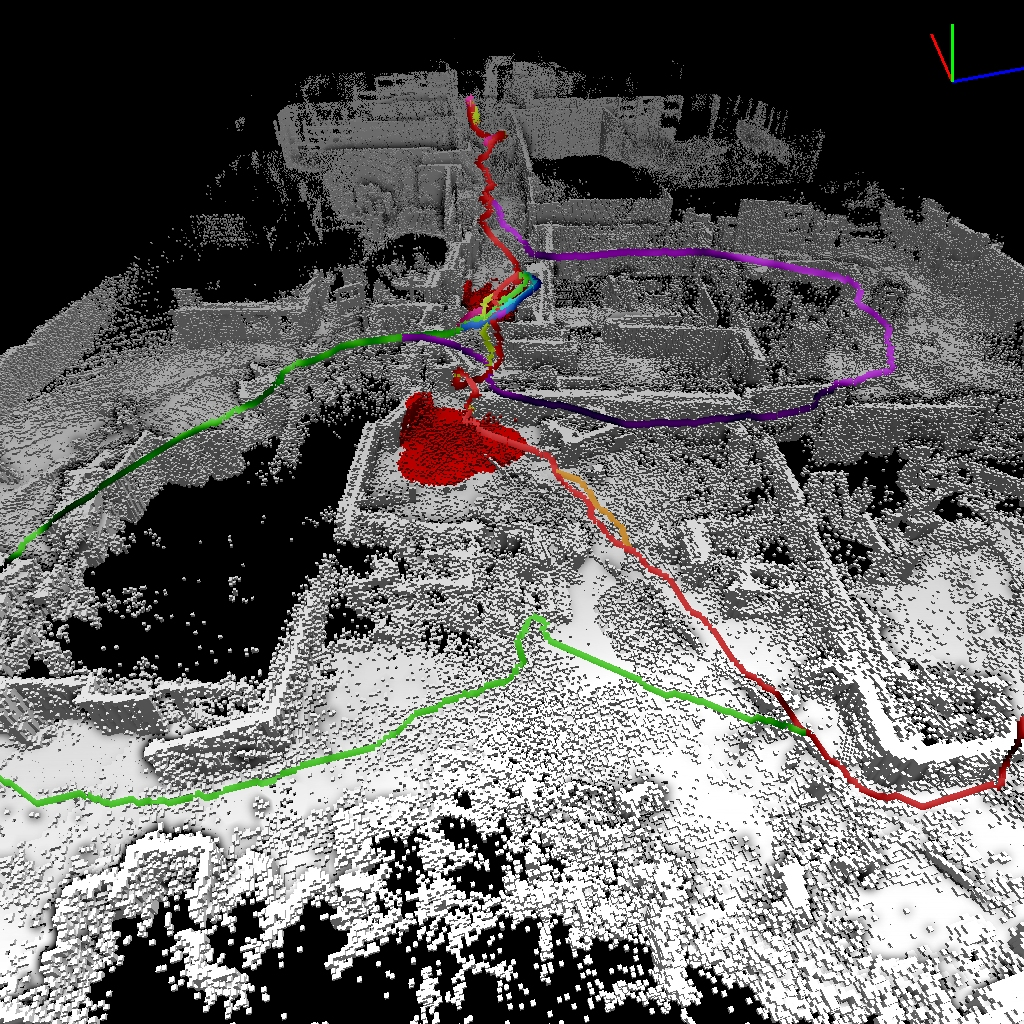
\includegraphics[width=0.4\columnwidth]{figures/fig-analysis-rendering.jpg}
    }
    \caption{The different paths are shown integrated into the rendering to provide a better awareness of the alternatives.}
    \label{fig:overview:analysis:paths}
\end{figure}
As autonomous robots are not yet used in emergency situations, it was not possible to obtain a dataset from a real-world disaster area. Hence we like to thank the IRIDeS, the CREATE, and the IRS institutes for their cooperation in retrieving three scans from the Fukushima Daiichi nuclear reactor in the aftermath of the 2011 meltdown. The equipment that was used to produce the scans are described in~\cite{journals/jfr/NagataniKOOYTNYKFK13}. As there had been hydrogen explosions and collapses in the building, it proved to be a valid and useful simulated real-world application case to test our proposed system.

Figure~\ref{fig:teaser:3} shows an overview of the scanned area with the selected entry area on the top in cyan, and the POI in green, on the bottom. No hazards were detected by the robots during the acquisition. The task was as follows: the \IC\ needs to find the shortest path between the entry and the POI. While traversing along the path, an imaginary rescuer would detect two hazard clouds (visible in red in Figure~\ref{fig:teaser:3}) and the system has to be able to react to this changing information as by requirement {\bfseries R2}.

Figure~\ref{fig:overview:analysis:paths} shows the rendering with all computed paths after the second hazard has been discovered. There is one class of paths (shown in purple) that evades the first hazard and another class (shown in green) that evades the second hazard. The parallel coordinates plot (Figure~\ref{fig:overview:analysis:pcp} makes it possible to detect a path that belongs to both classes as it has a maximum in the minimal distance to the hazard, while having a long path length (the selected path). In this snapshot of the SPLOM, Figure~\ref{fig:overview:analysis:scatter} shows the relationship between path length and the standard deviation of the support area and shows that the shorter the paths tend to pass through more unstable areas. The profile plot in Figure~\ref{fig:overview:analysis:profile} shows the prominence of the purple path as well.
